\section{Einleitung}

Wir programmieren einen \textit{Geometry Wars}\footnote{siehe~\cite[]{WikipediaGeometryWars}} Klon in C++.
Bei der Umsetzung orientieren wir uns teilweise an einer in der Industrie weit verbreiteten, von \textit{Gregory} in~\cite[]{Gre19} beschriebenen \textit{Game Engine Architektur}, reduzieren jedoch bewusst die Anzahl der Abstraktionsschichten und verzichten auf Systeme wie Tooling, Sound oder Scripting (vgl.~\cite[\textbf{Figure 1.16}, 39]{Gre19}), so dass die \textit{Hard Architecture}~\cite[]{RM04} einem Framework entspricht, welches Schnittstellen für benötigte Hardware und andere Subsysteme bereitstellt, die dem eigentlichen Spiel als technischer Unterbau dienen.
Das Spiel selber wird - als \textit{Black Box}~\cite[]{RB88} - von diesen Schnittstellen Gebrauch machen.\\

\begin{figure}[!h]
    \centering
    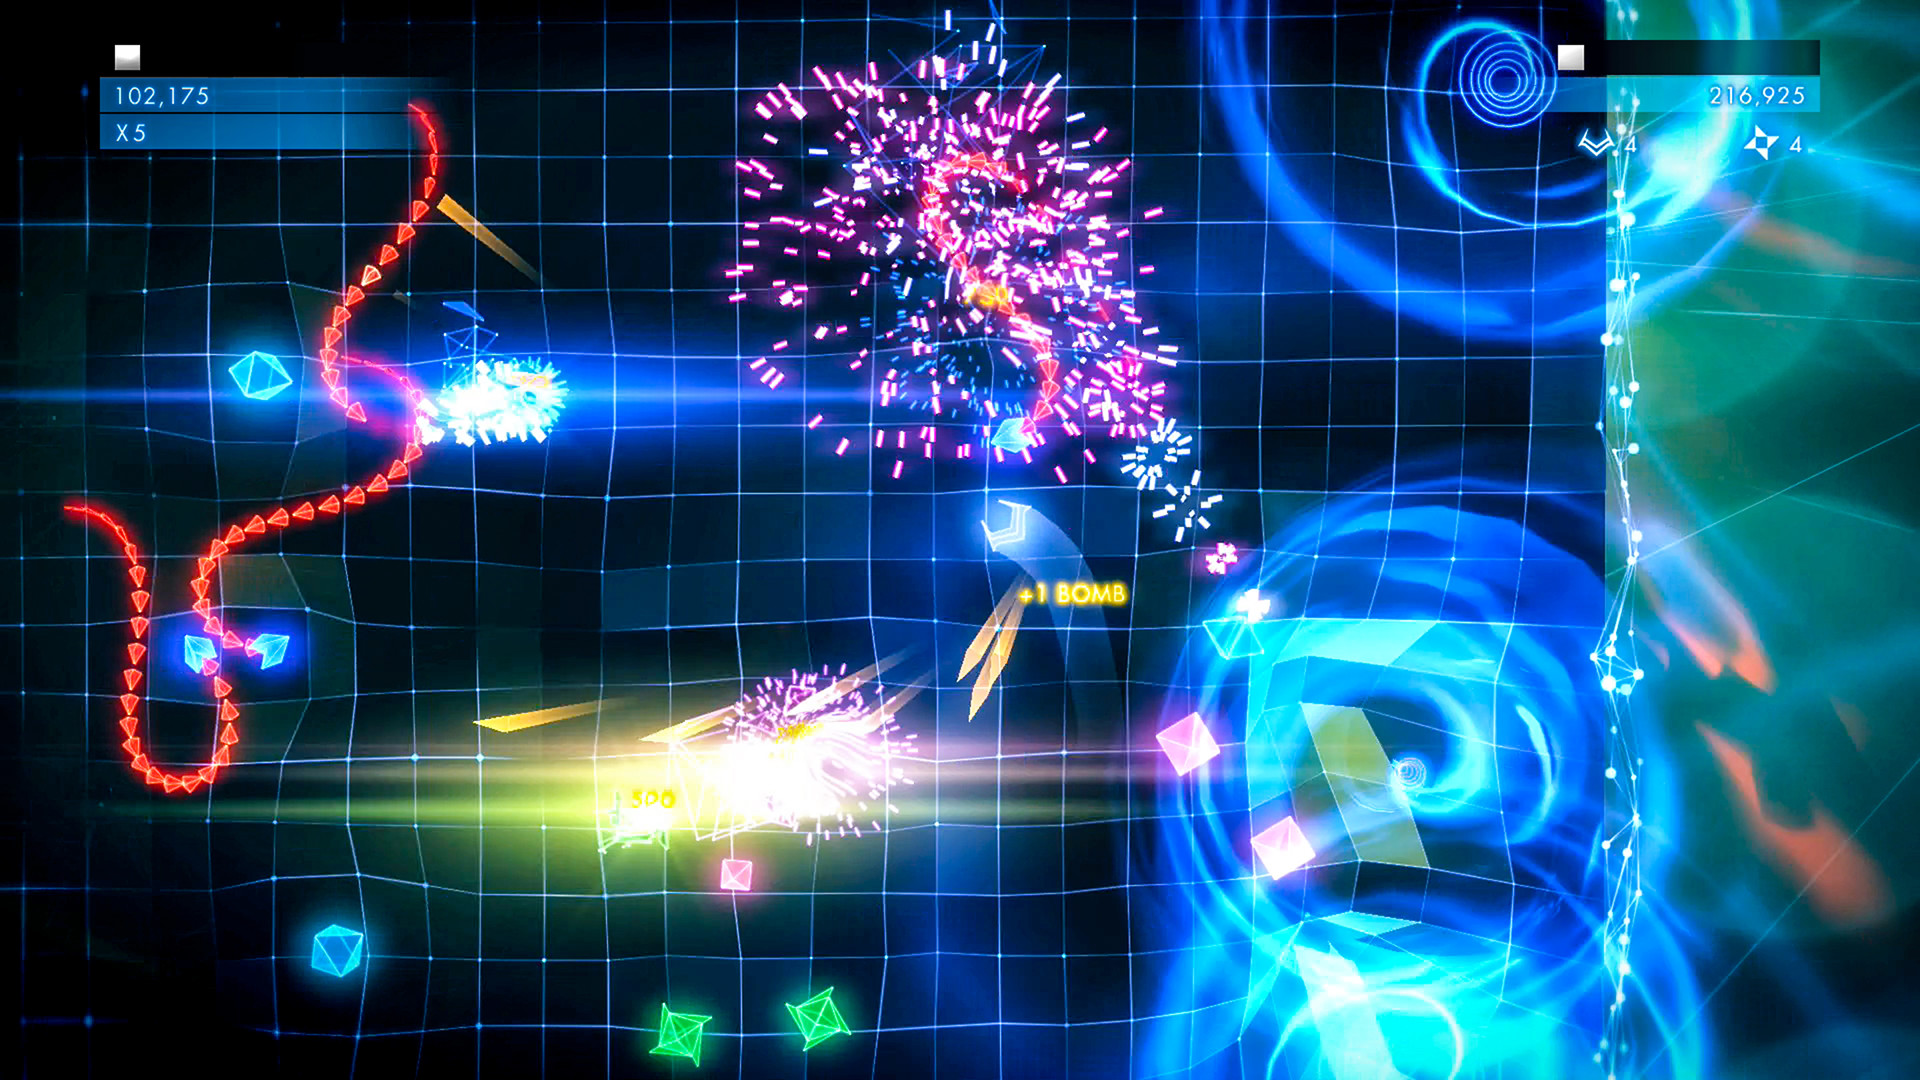
\includegraphics[width=1\columnwidth]{img/geometry_wars}
    \caption{Geometry Wars fand sich erstmals 2003 als Easter Egg in dem Spiel \textit{Project Gotham Racing} (Microsoft Game Studios). Aufgrund der großen Beliebtheit entstanden mehrere Nachfolger, zuletzt 2016 mit \textit{Geometry Wars 3: Dimensions Evolved} (Activision). (Quelle: Steam)}
    \label{fig:geometry_wars}
\end{figure}

In den nachfolgenden Abschnitten wird die Architektur von dem mit \textbf{helios}\footnote{
    Helios, der ``scharf vor allen mit strahlenden Augen umherblickt`` (\textit{Homers Ilias}, 14. Gesang), ist in der griechischen Mythologie der Sonnengott.
} getauften Framework vorgestellt.
Dabei berücksichtigen wir, dass es sich um einen in der Entwicklung befindlichen Prototypen handelt:
Die Software wird im Rahmen eines agilen \textit{Tracer Bullet Development}-Prozess~\cite[50 f.]{TH20} entwickelt.
Dadurch soll das Gesamtsystem verhältnis- und zweckmäßig angepasst werden können, woraus sich auch Anforderungen an die Architektur ableiten lassen.
In Abschnitt~\ref{sec:projektdaten} wird noch einmal gesondert auf die Anforderungen eingegangen. \\

\begin{figure}[!h]
    \centering
    
\includegraphics[width=0.5\columnwidth]{img/helios_logo}
    \caption{Das helios Projekt-Logo.}
    \label{fig:helios_logo}
\end{figure}


Wir betrachten auch Probleme und Schwierigkeiten, die bei der bisherigen Umsetzung aufgetaucht sind.
Diese ergeben sich u.a. durch den Umstand, dass das in vergleichsweise kurzer Zeit zu erstellende Softwareprodukt nicht nur anhand \textit{objektiver} Maße bewertet werden soll (etwa der Fehleranzahl, Software-Designentscheidungen, Kopplungsgrad der Objekte etc.), sondern auch anhand \textit{subjektiver} Maße~\cite[385]{Bal08}.\\
Zwar ist keine Klassifizierung des fertigen Produkts nach Nutzungsqualitätsmerkmalen wie bspw. ISO/IEC 9126 angedacht\footnote{bspw. ``Nutzungsqualität nach ISO/IEC 9126``,~\cite[466]{Bal08}; Studien und Untersuchungen u.a. bei~\cite[]{AZMK17},~\cite[]{Ber10}}.
Dennoch soll das Ergebnis nicht nur technisch ausgereift sein, sondern auch für den Anwender angenehm zu bedienen.
Dieses Nutzererlebnis wird im Weiteren formal eher unscharf, aber mit dem in der Spieleentwicklung etablierten Begriff des \textit{Game Feel}~\cite[]{Swi08} zusammengefasst: Einem möglichst \textit{angenehmen} und in jeglicher Hinsicht \textit{positiven Spielerlebnis}.

